\chapter{.tfc Bitstream Specification}
\label{chap:bitstream}

A video compression format is defined by its bitstream syntax. In this chapter, we document the .tfc container architecture, detailing its evolution across versions 1 through 5. We describe the header structure, 2-bit mode map bit-packing, run-length encoding (RLE), parameter quantization, and the v5 bounded-chunk streaming specification with audio encapsulation and frame rate preservation.

\section{Container Evolution Overview}
The .tfc format evolved across five distinct iterations to transition from an experimental research prototype to a bounded-memory, streamable media container:
\begin{itemize}
    \item \textbf{Version 1 (Monolithic Prototype):} Stored raw IEEE 754 floating-point parameter arrays and uncompressed mode maps for an entire video in a single monolithic header and payload structure.
    \item \textbf{Version 2 (Scene Segmentation):} Introduced scene-cut boundary detection, partitioning the timeline into variable-length temporal segments, each carrying its own mode map and payloads.
    \item \textbf{Version 3 (Tile-Native Storage \& Quantization):} Replaced floating-point parameter storage with uniformly quantized integer tables. Transitioned from per-pixel spatial addressing to tile-native scan orders, dramatically reducing header and index overhead.
    \item \textbf{Version 4 (Motion-Compensated Payloads):} Added signed motion offset vectors per tile to enable temporal warping prior to 1D regression, supporting general video presets.
    \item \textbf{Version 5 (Bounded Chunked Streaming Container):} Introduced independent fixed-window video chunks, record-level framing, CRC32 payload checksums, exact rational frame rate timing ($N/D$), and multiplexed audio stream preservation.
\end{itemize}

\section{Container Header Syntax}
All .tfc files commence with a 4-byte magic signature indicating the container version:
\begin{verbatim}
    'TFC1' | 'TFC2' | 'TFC3' | 'TFC4' | 'TFC5'
\end{verbatim}
In versions 1 through 4, the magic bytes are immediately followed by a 4-byte big-endian unsigned integer indicating the length $L_{\text{hdr}}$ of a UTF-8 encoded JSON header payload. In version 5, the container operates as a sequence of discrete binary chunks.

\begin{table}[h]
\centering
\small
\caption{Key Container Header Fields.}
\label{tab:header_fields}
\begin{tabular}{lll}
\toprule
\textbf{Field} & \textbf{Type} & \textbf{Description} \\
\midrule
\texttt{version} & Integer & Container version (1, 2, 3, 4, or 5). \\
\texttt{width} & Integer & Horizontal frame resolution in pixels ($W$). \\
\texttt{height} & Integer & Vertical frame resolution in pixels ($H$). \\
\texttt{frames} & Integer & Total number of video frames ($T$). \\
\texttt{tiling} & Integer & Spatial block dimension $B \times B$ ($1$ for per-pixel). \\
\texttt{color\_format} & String & Color representation (\texttt{"rgb"}, \texttt{"yuv444"}, \texttt{"yuv420"}). \\
\texttt{payload\_comp\_type} & Integer & Entropy codec (0: None, 1: zlib, 2: lzma, 3: zstandard). \\
\texttt{fps\_num}, \texttt{fps\_den} & Integer & Rational frame rate numerator and denominator (v5). \\
\texttt{has\_audio} & Boolean & Indicator of encapsulated audio bitstream (v5). \\
\bottomrule
\end{tabular}
\end{table}

\section{Mode Map Representation and Bit-Packing}
Because TimeFlowCodec assigns a discrete coding mode to every spatial unit (pixel or tile) across each color plane, compact mode representation is critical to prevent signaling overhead from dominating the bit budget.

\subsection{2-Bit Mode Assignments}
Each spatial unit is assigned one of four operational modes:
\begin{align*}
    00_2 \ (0) &\implies \textsc{Mode\_TFC\_Const} \quad (\text{Parameter } a) \\
    01_2 \ (1) &\implies \textsc{Mode\_TFC\_Linear} \quad (\text{Parameters } a, b) \\
    10_2 \ (2) &\implies \textsc{Mode\_FB\_Raw} \quad (\text{Raw sample vector } \mathbf{s}) \\
    11_2 \ (3) &\implies \textsc{Mode\_TFC\_Matrix} \quad (\text{Rank-1 factors } \mathbf{u}, \mathbf{v})
\end{align*}
These four states require exactly 2 bits of storage per unit. Four contiguous spatial units are packed into a single byte:
\begin{equation}
    \text{Byte} = (m_0 \ll 6) \mid (m_1 \ll 4) \mid (m_2 \ll 2) \mid m_3
\end{equation}
where $m_i \in \{0, 1, 2, 3\}$.

\subsection{Run-Length Encoding (RLE) of Mode Maps}
In screen recordings and presentation slide decks, large contiguous spatial regions (such as solid backgrounds, toolbars, or text margins) share identical constant or linear modes. 

To exploit this spatial coherence without incurring the overhead of a 2D transform, modern .tfc containers pass the packed 2-bit mode maps through a byte-oriented Run-Length Encoder:
\begin{itemize}
    \item A run of identical mode bytes is encoded as a 2-byte token: $\langle \text{ByteValue}, \text{RunLength} \rangle$.
    \item Runs exceeding 255 units are segmented into consecutive tokens.
\end{itemize}
For a $1920 \times 1080$ screen frame where $80\%$ of pixels are constant background, RLE reduces the mode map from approximately 518~KB to under 4~KB.

\section{Parameter Quantization}
A major architectural advancement introduced in v3 was the total elimination of raw floating-point numbers in the bitstream.

\subsection{Quantization of Intercept ($\hat{a}$)}
The intercept parameter $\hat{a}$ corresponds directly to the temporal base intensity. Because pixel intensities in digital video occupy the range $[0, 255]$, $\hat{a}$ is quantized to an 8-bit unsigned integer:
\begin{equation}
    a_{\text{quant}} = \text{clamp}\left(\lfloor \hat{a} + 0.5 \rfloor, 0, 255\right) \in \text{uint8}
\end{equation}

\subsection{Quantization of Slope ($\hat{b}$)}
The slope parameter $\hat{b}$ represents the per-frame intensity change:
\begin{equation}
    \Delta s = \hat{b} \cdot \Delta t
\end{equation}
Over a typical window of $T \le 120$ frames, physically plausible intensity shifts satisfy $|\hat{b}| \le 255 / T$.

To preserve fractional precision while using integer storage, $\hat{b}$ is scaled by a dynamic fixed-point factor $Q_b = 256$ and stored as a signed 16-bit integer:
\begin{equation}
    b_{\text{quant}} = \text{clamp}\left(\lfloor \hat{b} \cdot Q_b + 0.5 \rfloor, -32768, 32767\right) \in \text{int16}
\end{equation}
On decoding, the continuous reconstruction is evaluated in fixed-point or floating-point:
\begin{equation}
    \hat{s}_t = a_{\text{quant}} + \left(\frac{b_{\text{quant}}}{Q_b}\right) t
\end{equation}
This quantization strategy guarantees that parametric parameters require at most 3 bytes per pixel-channel over an entire temporal window, compared to $8$ bytes in raw float32 or $T$ bytes in uncompressed video.

\section{The Version 5 Bounded Chunked Streaming Architecture}
In versions 1 through 4, the entire video sequence was decoded into an in-memory NumPy array. For long 1080p or 4K videos, this caused memory consumption to scale linearly with video duration, quickly exhausting available system RAM.

Version 5 resolves this by introducing a \textit{bounded chunked container}:

\begin{figure}[t]
    \centering
    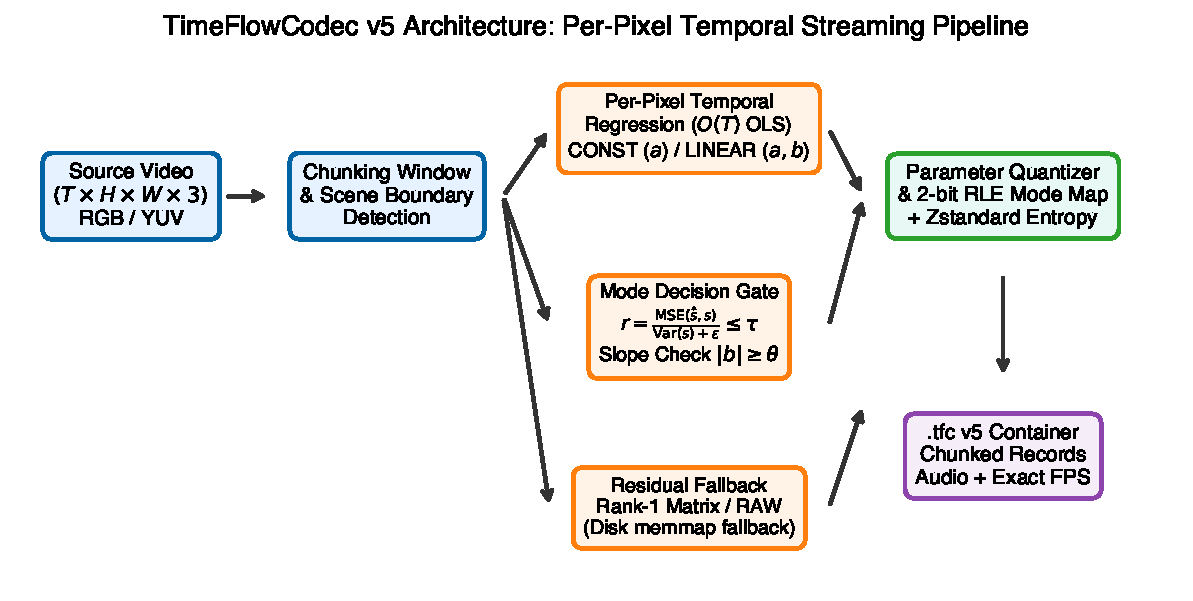
\includegraphics[width=\linewidth]{figures/tfc_architecture_v5.pdf}
    \caption{TimeFlowCodec version 5 streaming container layout and decoding pipeline, featuring chunked framing, checksum verification, audio encapsulation, and bounded memory playback.}
    \label{fig:v5_architecture}
\end{figure}

As shown in Figure~\ref{fig:v5_architecture}, a v5 stream comprises:
\begin{enumerate}
    \item \textbf{Master Container Header:} Contains overall video dimensions, rational frame rate (e.g., $30000 / 1001$ for $29.97\text{ FPS}$), audio track descriptors, and default chunk window sizes (typically $T_{\text{chunk}} = 24$ to $48$ frames).
    \item \textbf{Sequence of Self-Contained Chunks:} Each chunk encapsulates exactly $T_{\text{chunk}}$ frames across all three color channels. A chunk begins with a 4-byte chunk length and 4-byte CRC32 checksum, followed by the compressed plane payloads.
    \item \textbf{Audio Record Streams:} Raw AAC or Opus audio packets extracted from the source media are interleaved between video chunks, preserving exact audio-video synchronization without re-encoding.
    \item \textbf{Atomic Writers and Truncation Guards:} Writers construct chunks atomically using temporary storage, verifying payload size bounds and CRC integrity before committing records to disk.
\end{enumerate}

\section{Entropy Coding Layer}
Following RLE mode-packing and parameter quantization, all byte buffers are passed to an entropy coding stage. TimeFlowCodec supports four entropy algorithms configured via \texttt{payload\_comp\_type}:
\begin{itemize}
    \item \texttt{COMP\_NONE} (0): Uncompressed raw binary buffers.
    \item \texttt{COMP\_ZLIB} (1): Standard DEFLATE compression.
    \item \texttt{COMP\_LZMA} (2): High-ratio Lempel-Ziv-Markov chain compression.
    \item \texttt{COMP\_ZSTD} (3, default): Modern Zstandard compression~\cite{collet2015zstandard} operating at level 10, providing an optimal balance of fast decompression throughput (exceeding $1.2\text{ GB/s}$) and high compression ratio on structured binary payloads.
\end{itemize}
